%%%%%%%% ICML 2019 EXAMPLE LATEX SUBMISSION FILE %%%%%%%%%%%%%%%%%

\documentclass{article}

% Recommended, but optional, packages for figures and better typesetting:
\usepackage{microtype}
\usepackage{graphicx}
\usepackage{subfigure}
\usepackage{amsmath}
\usepackage{amsfonts}
\usepackage{enumitem}
\usepackage{amsthm}
\newtheorem{theorem}{Theorem}
\usepackage{xcolor}
\usepackage{natbib}
\usepackage{booktabs} % for professional tables
% hyperref makes hyperlinks in the resulting PDF.
% If your build breaks (sometimes temporarily if a hyperlink spans a page)
% please comment out the following usepackage line and replace
% \usepackage{icml2019} with \usepackage[nohyperref]{icml2019} above.
\usepackage{hyperref}

% Attempt to make hyperref and algorithmic work together better:
\newcommand{\theHalgorithm}{\arabic{algorithm}}

% Use the following line for the initial blind version submitted for review:
\usepackage{icml2019}

% If accepted, instead use the following line for the camera-ready submission:
%\usepackage[accepted]{icml2019}

% The \icmltitle you define below is probably too long as a header.
% Therefore, a short form for the running title is supplied here:
\icmltitlerunning{Compositional Invariance Constraints for Graph Embeddings}

% Blackboard bold
\def\P{\mathbb{P}}
\def\C{\mathbb{C}}
% Numbers
\def\R{\mathbb{R}}
\def\Z{\mathbb{Z}}
\def\Q{\mathbb{Q}}
\def\N{\mathbb{N}}

\newcommand{\G}{\mathcal{G}}
\newcommand{\V}{\mathcal{V}}
\newcommand{\E}{\mathcal{E}}
\newcommand{\T}{\mathcal{T}}
\newcommand{\A}{\mathcal{A}}
\newcommand{\enc}{\textsc{enc}}
\newcommand{\compenc}{\textsc{c-enc}}

% Boldface used for vector notation
\def\I{\mathbf{I}}
\def\e{\mathbf{e}}
\def\r{\mathbf{r}}
\def\m{\mathbf{m}}
\def\o{\mathbf{o}}
\def\x{\mathbf{x}}
\def\p{\mathbf{p}}
\def\u{\mathbf{u}}
\def\v{\mathbf{v}}

% Other
\def\defeq{\dot=}
\newcommand\norm[1]{\left\lVert#1\right\rVert} % Norm
\newcommand{\red}{\textcolor{red}}
\DeclareMathOperator*{\argmin}{\arg\!\min}
\DeclareMathOperator*{\argmax}{\arg\!\max}
\newcommand{\xhdr}[1]{{\noindent\bfseries #1}.}
\newcommand{\cut}[1]{}
\newcommand{\CITE}{\textcolor{red}{CITE}}
\newcommand{\will}{\textcolor{cyan}}
\newcommand{\mb}{\mathbf}
\newcommand{\removelatexerror}{\let\@latex@error\@gobble}
\begin{document}

\twocolumn[
\icmltitle{Compositional Invariance Constraints for Graph Embeddings}

% It is OKAY to include author information, even for blind
% submissions: the style file will automatically remove it for you
% unless you've provided the [accepted] option to the icml2019
% package.

% List of affiliations: The first argument should be a (short)
% identifier you will use later to specify author affiliations
% Academic affiliations should list Department, University, City, Region, Country
% Industry affiliations should list Company, City, Region, Country

% You can specify symbols, otherwise they are numbered in order.
% Ideally, you should not use this facility. Affiliations will be numbered
% in order of appearance and this is the preferred way.
\icmlsetsymbol{equal}{*}

\begin{icmlauthorlist}
\icmlauthor{Aeiau Zzzz}{equal,to}
\icmlauthor{Bauiu C.~Yyyy}{equal,to,goo}
\icmlauthor{Cieua Vvvvv}{goo}
\icmlauthor{Iaesut Saoeu}{ed}
\icmlauthor{Fiuea Rrrr}{to}
\icmlauthor{Tateu H.~Yasehe}{ed,to,goo}
\icmlauthor{Aaoeu Iasoh}{goo}
\icmlauthor{Buiui Eueu}{ed}
\icmlauthor{Aeuia Zzzz}{ed}
\icmlauthor{Bieea C.~Yyyy}{to,goo}
\icmlauthor{Teoau Xxxx}{ed}
\icmlauthor{Eee Pppp}{ed}
\end{icmlauthorlist}

\icmlaffiliation{to}{Department of Computation, University of Torontoland, Torontoland, Canada}
\icmlaffiliation{goo}{Googol ShallowMind, New London, Michigan, USA}
\icmlaffiliation{ed}{School of Computation, University of Edenborrow, Edenborrow, United Kingdom}

\icmlcorrespondingauthor{Cieua Vvvvv}{c.vvvvv@googol.com}
\icmlcorrespondingauthor{Eee Pppp}{ep@eden.co.uk}

% You may provide any keywords that you
% find helpful for describing your paper; these are used to populate
% the "keywords" metadata in the PDF but will not be shown in the document
\icmlkeywords{Machine Learning, ICML}

\vskip 0.3in
]

% this must go after the closing bracket ] following \twocolumn[ ...

% This command actually creates the footnote in the first column
% listing the affiliations and the copyright notice.
% The command takes one argument, which is text to display at the start of the footnote.
% The \icmlEqualContribution command is standard text for equal contribution.
% Remove it (just {}) if you do not need this facility.

%\printAffiliationsAndNotice{}  % leave blank if no need to mention equal contribution
\printAffiliationsAndNotice{\icmlEqualContribution} % otherwise use the standard text.

\begin{abstract}
 Learning high-quality node embeddings is a key building block for machine learning models that operate on graph data, such as social networks and recommender systems. However, existing graph embedding techniques are unable to cope with fairness constraints, e.g., ensuring that the learned representations do not correlate with certain attributes, such as age or gender. Here, we introduce an adversarial framework to enforce fairness constraints on graph embeddings. Our approach is {\em compositional}---meaning that it can (optionally) enforce multiple different fairness constraints during inference. Experiments on standard knowledge graph and recommender system benchmarks highlight the utility of our proposed framework. 
\end{abstract}
\section{Introduction}
Learning low-dimensional embeddings of the nodes in a graph is a fundamental technique underlying state-of-the-art approaches to link prediction and recommender systems \cite{cai2018comprehensive,hamilton2017representation}. 
However, in many applications---especially those involving social graphs---it is desirable to exercise control over the information contained within these learned node embeddings. 
For instance, we may want to ensure that recommendations are fair or balanced with respect to certain attribtues (e.g., that they do not depend on a user's race or gender) or we may want to ensure privacy by not exposing certain attributes through learned node representations. 
In this work we investigate the feasibility of enforcing such {\em invariance constraints} on (social)  graph embeddings. 

While enforcing invariance constraints on general classification models \cite{chouldechova2017fair,gajane2017formalizing,kamishima2012fairness,madras2018learning,zemel2013learning} and collaborative filtering algorithms \cite{yao2017new} has received considerable attention in recent years, these techniques have yet to be considered within the context of graph embeddings---a setting that introduces particular challenges due to the non-i.i.d. and non-Euclidean nature of relational, graph data. 

Moreover, in the case of social graphs and large-scale recommender systems, it is often the case that there are many {\em possible} sensitive attributes that we {\em may} want to enforce invariance constraints over.
Previous work on enforcing invariance (or ``fairness'') in social applications has generally focused on situations that involve one sensitive attribute (e.g., age in the context of credit or loan decisions; \citet{zemel2013learning}), but in the context of social graph embeddings there can be an extremely large number of possible sensitive attributes. In fact, {\em we may even want to be fair with respect to the existence of individual edges.}
For instance, a user on a social networking platform might want that platform's recommender system to ignore the fact that they are friends with a certain other user, or that they engaged with a particular piece of content. 
%Allowing users to request invariance with respect to individual social relationships would provide an avenue to give users  power over their 

\xhdr{Present work}
We introduce an adversarial framework to enforce {\em compositional} fairness constraints on graph embeddings.
The key idea behind our approach is that we learn a set of {\em adversarial filters} that remove information about particular sensitive attributes.
Crucially, each of these learned filters can be {\em optionally} applied after training, so the model can flexibly generate embeddings that are invariant with respect to different sets of sensitive attributes. 
Our work builds upon the success of recent adversarial approaches to fairness \cite{zemel2013learning}, disentanglement \cite{mathieu2016disentangling}, and transfer learning \cite{madras2018learning}---extending these approaches to the domain of graph representation learning and introducing new algorithmic techniques to accommodate compositional constraints during inference.  

\cut{
Machine Learning on graph structured data has seen a tremendous rise in recent years. This is largely due to the ubiquity of data that can be naturally modeled as graphs i.e. recommendation systems, biological protein-protein networks, and social networks to name a few \cite{battaglia2018relational}. Indeed, even typical images can be viewed as a graph with an explicit grid structure which is a key property exploited by convolutional neural networks. However, in data where such grid structure is not readily found the central problem remains on how to incorporate information about the graph structure into a machine learning algorithm. In contrast with previous approaches, representation learning on graphs can be thought of as a machine learning task where the goal is to learn low dimensional embeddings of either nodes or subgraph information that are optimized to reflect the geometry of the original graph \cite{DBLP:journals/corr/abs-1709-05584}. 

Learning high quality representations is one of the primary objectives of machine learning research especially in domains such as natural language processing where word embeddings are a crucial building block for language models. An exciting new direction of research has shown that adversarial learning can be leveraged to not only learn better representations \cite{P18-1094} but to encode certain desirable properties \cite{P18-1152}. The focus of this research proposal is to use adversarial machine learning to learn representations from graph structured data. One direct consequence of this viewpoint is that algorithmic fairness can be easily expressed through these desirable invariance properties. This is especially important today as information systems are increasingly reliant on statistical inference and learning to render all sorts of decisions, including the setting of insurance rates,
the targeting of advertising, and the issuing of bank loans. As a result, it is imperative that these models are devoid of algorithmic bias and do not discriminate between groups or individuals. Furthermore, previous approaches to enforcing fairness, especially through an adversarial lens, have been limited to images and language but graph data introduces new complications due to its structured non-Euclidean nature and the fact that the datapoints are not i.i.d.
}
\section{Related work}

Our contribution is at the intersection of research on (social) graph embedding, algorithmic fairness, and adversarial learning.

\subsection{Graph embedding}
At the core of our proposed methodology is the notion of learning low-dimensional embeddings of graph-structured data.
Graph embedding techniques have a long history in the social sciences, with connections to early research on ``sociograms'' (small hand-constructed social networks) and latent variable models of social interactions \cite{faust1988comparison,majone1972social}.
The key motivation behind these early works---which continues to permeate and influence even recent work in the area---is the idea that the likelihood of observed social interactions can be approximated by geometric relationships in some underlying latent, social space. 

In more recent years, the task of embedding graph-structured data has received increasing attention from the machine learning and data mining communities \cite{cai2018comprehensive,hamilton2017representation}. 
Generally, the goal of these works is to map graph nodes to low-dimensional vector embeddings, such that the original graph can be (approximately) reconstructed from these embeddings.
Traditional approaches to this problem include Laplacian eigenmaps \cite{belkin2002laplacian} and matrix factorization techniques \cite{ng2001spectral}, with recent years witnessing a surge in methods that rely on random-walk based objectives \cite{grover2016node2vec,perozzi2014deepwalk}, deep autoencoders \cite{wang2016structural}, and graph neural networks \cite{hamilton2017inductive,kipf2016variational}. 

Learned graph embeddings can be used for a wide variety of tasks, including node classification, relation prediction, and clustering \cite{hamilton2017representation}.
Here, we focus on the relation prediction task, i.e., using the learned representations to predict previously unobserved relationships between the input nodes.
The relation prediction task is exceptionally general---for example, it generalizes basic recommender systems, knowledge base completion, and even node classification.\footnote{For instance, one can simply associate each class label with a node and define edge to these nodes as indicating class membership}
Moreover, the majority of graph embedding approaches use a relation prediction loss to train the representations \cite{cai2018comprehensive},
which makes this setting a natural focus for our exploration of fairness. 

\subsection{Algorithmic fairness}\label{sec:relatedfair}
Unlike previous research on graph embedding, in this work we focus on the challenge of enforcing fairness constraints on the learned representations. 
Recent work on fairness in machine learning, including work on fairness in collaborative filtering, involves making predictions that are balanced or invariant with respect to certain sensitive variables (e.g., age or gender) \cite{chouldechova2017fair,gajane2017formalizing,kamishima2012fairness,madras2018learning,zemel2013learning,yao2017new}. 
Formally, in the standard ``fair classification'' setting we consider a data point $\mb{x} \in \mathbb{R}^n$, its class label $y \in \mathcal{Y}$, and a binary sensitive attribute $a \in \{0,1\}$ (e.g., indicating gender). 
The high-level goal is then to train a model to predict $y$ from $\mb{x}$, while making this prediction invariant or fair with respect to $a$ \cite{madras2018learning}.
There are many specific definitions of fairness, such as whether fairness refers to parity or satisfying certain preferences (see \cite{gajane2017formalizing} for a detailed discussion). 
In the context of fair machine learning, our core contribution is motivating, implementing, and evaluating an approach to enforce fairness within the context of graph embeddings.
There are a number of complications introduced by this setting---for instance, rather than one classification task, we instead have thousands or even millions of interdependent edge relationships. 

\section{Preliminaries}

We consider the general case of embedding a hetereogenous or multi-relational (social) graph $\G = (\V, \E)$, which consists of set of directed edge triples $e=\langle u, r, v \rangle \in \E$, where $u, v \in \V$ are nodes and $r \in \R$ is a relation type.
We further assume that each node is of a particular type, $\T \subseteq \V$, and that relations may have constraints regarding the types of nodes that they can connect. 

\xhdr{Relation prediction}
The general {\em relation prediction} task on such a  graph is as follows.
Let $\E_{\textrm{train}}\subset \E$ denote a set of observed {\em training} edges and let $\bar{\E} = \{\langle v_i, r, v_j \rangle : v_i, v_j \in \V, r \in R\} \setminus \E$ denote the set of {\em negative} edges that are not present in the true graph $\G$.
Given $\E_{\textrm{train}}$, we aim to learn a scoring function $s$ such that
\begin{equation}\label{eq:score}
    s(e) > s(e'), \forall e \in \E, e' \in \bar{\E}.
\end{equation}
In other words, the learned scoring function should (ideally) score any true edge higher than any negative edge. 

\xhdr{Embedding-based models}
In the context of graph embeddings, we aim to solve this relation prediction task by learning a function $\enc : \V \mapsto \mathbb{R}^d$ that maps each node $v \in \V$ to an embedding $\mb{z}_v = \enc(v)$.
In this case, the signature of the score function becomes $s_\Theta : \mathbb{R}^d \times \R \times \mathbb{R}^d \mapsto \mathbb{R}$, i.e., it takes two node embeddings $\mb{z}_u, \mb{z}_v \in \mathbb{R}^d$ as input and uses these embeddings to score the likelihood that an edge $e=<u, r, v>$ exists in the graph. 
Generally, the intuition in embedding-based approaches is that the distance between two node embeddings should encode the likelihood that there is an edge between the nodes, with the distance computation depending on the relation in question.  
For instance, a concrete example of this embedding-based approach is the TransE \cite{bordes2013translating} model, where each relation $r \in \R$ is associated with an embedding $\mb{r} \in \mathbb{R}^{d}$ and the scoring function is defined as
\begin{align}
    s(\mb{z}_u, r, \mb{z}_v) &=  - \|\mb{z}_u^\top + \mb{r} - \mb{z}_v\|_2,
\end{align}
i.e., the likelihood of a relation holding between two nodes is proportional to their distance, after translating one of the node embeddings by a learned relation embedding. 
TransE is just on many possible instantiations of this general approach, and many scoring functions have been proposed in recent years---including RESCAL \cite{nickel2011three}, ComplexE \cite{trouillon2016complex} and TransD \cite{ji2015knowledge}.
The framework we discuss below is compatible with any of these scoring functions, as long as they are differentiable and depend on the input nodes only through their embeddings. 

Graph embedding models of this variety are usually optimized using {\em noise contrastive estimation}, where the loss over a batch of edges 
$\E_{\textrm{batch}} \in \E_{\textrm{train}}$ is given by:
\begin{equation}\label{eq:genericloss}
    \sum_{e \in \E_{\textrm{edge}}} L_{\textrm{edge}}(s(e), s(e^{-}_1), ..., s(e^{-}_m)),
\end{equation}
where $L_{\textrm{edge}}$ is a per-edge loss function and $e^{-}_1, ..., e^{-}_m \in \bar{\E}$ are ``negative samples'', i.e., randomly sampled edges that do not exist in the graph.
Intuitively, loss functions of this form attempt to maximize the likelihood of true edges compared to the negative samples. 


\xhdr{Fairness}
Lastly, in order to incorporate the notion of fairness into the graph embedding setup, we assume that for exactly one node type $\T^*$, all nodes of this type, i.e. all $u \in \T^*$, have $K$ categorical sensitive attributes, $h(u) = a^k_u \in \A_k, k=1...,K$, and for simplicity, we assume that there are no other features or attributes associated with the nodes and edges in the graph.\footnote{Though this assumption can easily be relaxed.}
The challenge in enforcing fairness is thus to ensure that the learned node embeddings, $\mb{z}_u$, are not biased or unfair with respect to these sensitive attributes---a point which we formalize in the next section. 
For example, in a simple social recommendation setting, we may have one type of node, $\T = \{\texttt{users}\}$ and one type of relation, $\mathcal{R} = \{\texttt{friends}\}$.
In the basic graph embedding setting, our goal would be to learn embeddings of the users, which we could use to make friend recommemndations. 
However, in the case of enforcing fairness, we might further assume that all the users have a categorical attributes indicating their age and gender, and our goal would to be recommend friends in such a way that does not depend on these attributes. 

\section{Invariant Graph Embeddings}

We first motivate and argue in favor of particular form of ``fairness'' (or rather {\em invariance}) within the context of graph embeddings.
Following this, we outline our compositional and adversarial approach for enforcing these invariance constraints on graph embeddings. 

\subsection{Pragmatic fairness as invariance}

As noted in Section \ref{sec:relatedfair}, there are a multitude of definitions of algorithmic fairness in the literature---each definition with its own benefits and drawbacks.
Thus, rather than developing yet another new metric---or diving into thorny debates regarding the pros and cons of different formulations---in this work we instead consider a simple, user-centric formulation within the context of social graph embeddings.
Using gender as an example of a sensitive attribute and movie recommendation as an example relation prediction task, our approach is guided by the following question: {\em If one gives a user a button that says ``Please ignore my gender when recommending movies'', what does a user expect from the system after this button is pressed?}
Here, we accept it as non-controversial that the expectation from the user is that recommendation does not depend in any way on their gender, i.e., that the recommendation would be the same regardless of their gender.
Formally, given a user $u$, this expectation amounts to an assumption of independence, 
\begin{equation}\label{eq:edgeind}
  s(e) \perp a_u \qquad \forall v \in \V, r \in \R
\end{equation}
between the recommendation---i.e., the score of the edge, $s(e) = s(\langle \mb{z}_u, r, \mb{z}_v\rangle)$---and the sensitive attribute $a_u$.

One issue in directly enforcing Equation \eqref{eq:edgeind} is that there are many (potentially millions) of possible edges that we might want to score for every node $u \in \T^*$, making it intractable to enforce independence on each of these decisions individually.
However, if we assume that the score function $s\langle \mb{z}_u, r, \mb{z}_v \rangle)$ depends on $u$ only through $u's$'s embedding, $\mb{z}_u$, then we can guarantee the independence in Equation \eqref{eq:edgeind} for all edge predictions by enforcing what we call {\em representational invariance}:
\begin{equation}\label{eq:repinvar}
    \mb{z}_u \perp a_u \:\: \forall u \in \V.
\end{equation}
In other words, we can simply ensure that the node embeddings themselves are invariant to the sensitive attributes/%, which ensures information about the sensitive attributes is not available to any downstream predictions made using these embeddings. 
Note that this invariance assumption is equivalent to requiring that the mutual information $I(\mb{z}_u, a_u)$ is $0$.

Generalizing to the setting of multiple sensitive attributes, for a given set of sensitive attributes $S \subseteq \{1, ..., K\}$, we would require that
\begin{equation}\label{eq:multirepinvar}
     I(\mb{z}_u, a^k_u) =0, k\in S, \forall u \in \V,
\end{equation}
which amounts to the assumption of $S$ independent invariance constraints on the $S$ distinct sensitive attributes.\footnote{Note that this does not necessarily imply ``subgroup fairness'' with respect to the joint distribution of the sensitive attributes \cite{kearns2017preventing}.}
Importantly, {\em we assume that the set $S$ is not fixed} (e.g., different users might request different invariance constraints). 

In the language of algorithmic fairness, the representational invariance of Equation \eqref{eq:repinvar} implies that traditional demographic parity constraints are satisfied on the sensitive attributes and recommendations.
Formally, for any node $u \in \T^*$ and any pair of sensitive attribute values $a', a \in \A$, Equation \ref{eq:repinvar} guarantees that $\forall \alpha \in \mathbb{R}, v \in \V$:
\begin{equation}
    P( s(e) > \alpha | a_u = a) =  P( s(e) > \alpha | a_u = a') \:\: ,
\end{equation}
which amounts to a demographic parity constraint, assuming that edge predictions are made by some threshold on the scoring function $s$.
Many drawbacks of demographic parity have been outlined in the literature \cite{gajane2017formalizing}.
However, in this work, when considering the pragmatic perspective of user expectations, representational invariance (and thus demographic parity) appears to be the most reasonable option: for instance, when a user says that they do not want their movie recommendations to depend on their gender, then they expect exactly that (and not some more complicated or nuanced notion of group fairness).  
\cut{
Of course, this is not to say that demographic parity is the {\em right} form of fairness in all settings, as in some instances (e.g., insurance decisions) we may want to enforce equalize odds \CITE\ or in other instances we may want to ensure fairness with respect to prediction accuracies across subgroups \CITE.
Here, we simply argue that representational invariance is a natural constraint to enforce if we want to make embedding-based recommendations that do not depend on certain user attributes.  
}

% where we consider the more challenging task of accommodating flexible or dynamic fairness constraints. Such constraints can optionally be enforced at test time and intuitively has the effect of giving back power or agency to users: they get to decide if and how ``fair" the recommendations made are to them. 

\subsection{Model definition}

In this work, we enforce representational invariance constraints on the node embeddings (Equation \ref{eq:multirepinvar}) by introducing an adversarial loss and a technique to ``filter'' the embeddings generated by the $\enc$ function.
Note, again, that a unique challenge here is that $S$---the set of sensitive attributes we want to be invariant with respect to---is not  fixed across nodes, i.e., we may want to enforce invariance on different sets of sensitive attributes for different nodes. 

Note also that the framework presented in this section is quite general and can function with arbitrary combinations of base node embedding functions $\enc$ and edge-prediction losses $L_{\textrm{edge}}$ (see Equation \ref{eq:genericloss}).
We discuss three concrete instantiations of this framework in Section \ref{sec:experiments}.

\xhdr{Compositional encoder}
The first key component of our model is generalizing the $\enc$ embedding function to optionally ``filter'' out the information about certain sensitive attributes. 
In particular, for every sensitive attribute $k \in \{1, ..., K\}$ we define a filter function $f_k : \R^d \mapsto \R^d$ that is trained to remove the information about the $k$th sensitive attribute. 
If we want the node embedding to be invariant w.r.t. some set of sensitive attributes $S \subseteq \{1,...,K\}$, we then generate its embedding by ``composing'' the output of the $|S|$ filtered embeddings using a {\em compositional encoder}:
\begin{equation}
    \compenc(u, S) = \frac{1}{|S|}\sum_{k \in S}f_k(\enc(u))
\end{equation}

\xhdr{Adversarial loss}
To train the compositional encoder, we employ an adversarial regularizer, which penalizes the node embeddings for containing information about the sensitive attributes.
For each sensitive attribute $k \in K$, we define a discriminator $D_k : \mathbb{R}^{d} \times \A_k \mapsto [0,1]$, which attempts to predict the $k$th sensitive attribute from the node embeddings. 
Assuming we are given an edge-prediction loss function $L_\textrm{edge}$ (as in Equation \ref{eq:genericloss}), we can then define our new adversarially regularized per-edge loss as
\begin{align}\label{eq:loss}
    L(e) = &L_{\textrm{edge}}(s(e), s(e^{-1}_1), ..., s(e^{-1}_m)) \nonumber \\ &+ \lambda \sum_{k \in S}\sum_{a^k \in \A_k}\log(D_k(\compenc(u, S), a^k)),
\end{align}
where $\lambda$ is a hyperparameter controlling the strength of the adversarial regularization and $S \subseteq \{1,...,K\}$ is the set of sensitive attributes that we are enforcing invariance on for this edge. 
To optimize this loss in a minibatch setting, we alternate between two types of stochastic gradient descent updates: (1) $T$ minibatch updates maximizing $L(e)$ with respect to $\compenc$ (with all the $D_k$ fixed), and (2) $T'$ minibatch updates  minimizing $-L(e)$ with respect to $D_k, k=1...,K$ (with $\compenc$ fixed).  



\begin{figure}
    \centering
    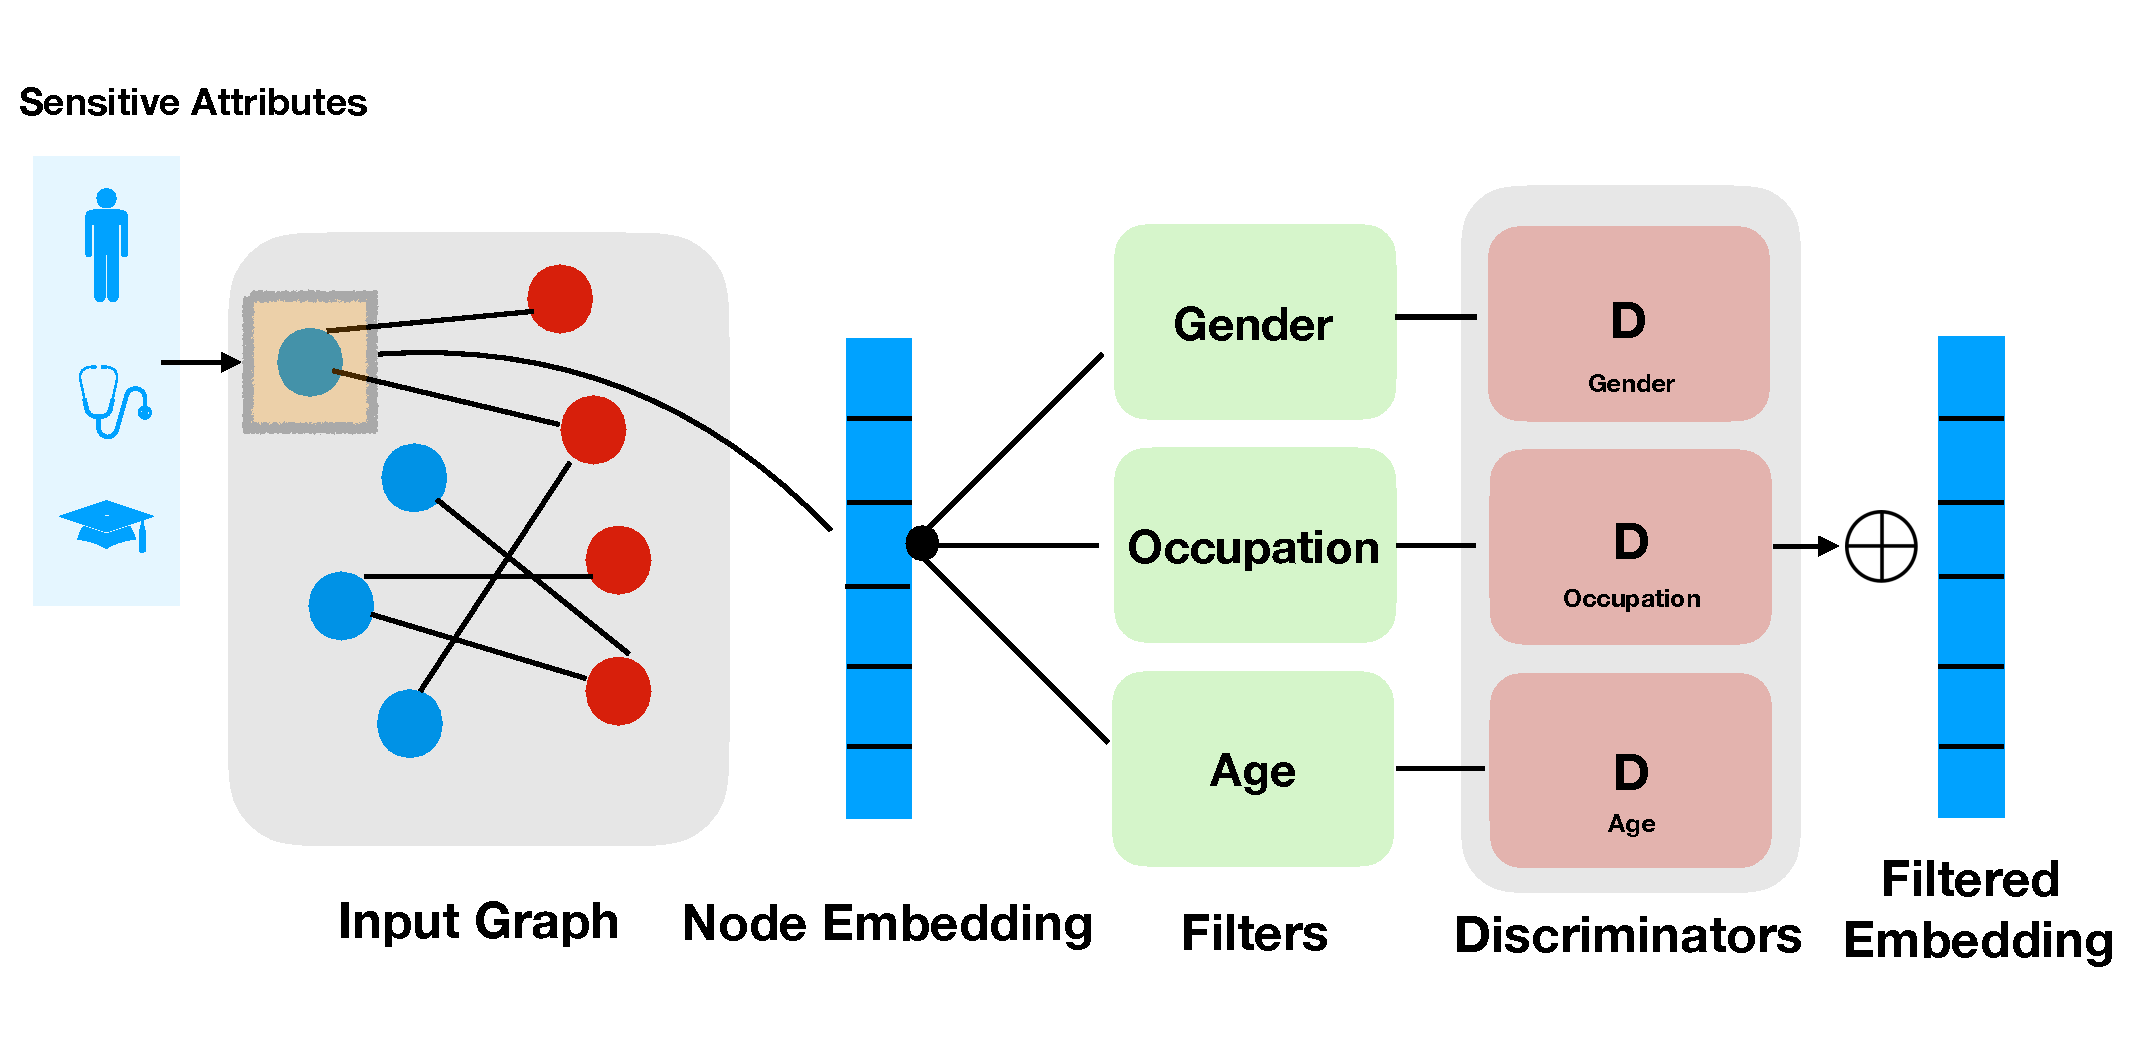
\includegraphics[width=1\linewidth]{icml2019_style/paper/plots/LightningTalk-Graphic.pdf}
    \vspace{-5mm}
    \caption{Compositional Adversary Architecture}
    \label{arch}
\end{figure}

\xhdr{Theoretical intuitions}
For clarity and simplicity, we consider the case of a single binary sensitive attribute, with the theoretical intuitions naturally generalizing to the multi-attribute and multi-class settings.
Assuming a single binary sensitive attribute $a_k$, by simple application of Proposition 2 in \citet{goodfellow2014generative}, we have:
\begin{theorem}
If $\compenc$ and $D_k$ have enough capacity, $T'$ is large enough so that $D_k$
is allowed to reach its optimum on $-L(e)$ (with $\compenc$ fixed), and $\compenc$ is optimized according to $L(e)$ (with $D$ fixed), then $I(\mb{z}_u, a_u) \rightarrow 0, \forall u \in \T^*$ as $\lambda \rightarrow \infty$. 
\end{theorem}
That is, if we increase the weight of the adversarial regularizer to infinity, the equilibrium of the minimax game in Equation \eqref{eq:loss} occurs when there is zero mutual information between the sensitive attribute and the embeddings. 
Of course, as $\lambda \rightarrow \infty$ trivial solutions to thie game exist (e.g., $\compenc$ simply outputting a constant value) and in practice setting $\lambda < \infty$ leads to a tradeoff between performance on edge prediction and representational invariance.
Theorem 1 holds as a consequence of Proposition 2 in \citet{goodfellow2014generative} if we simply replace the task of distinguishing real/fake data by classifying a binary sensitive attribute. 
\section{Experiments}\label{sec:experiments}

We investigated the impact of enforcing invariance on graph embeddings using three  datasets: Freebase15k-237\footnote{\tiny{\url{www.microsoft.com/en-us/download/details.aspx?id=52312}}}, MovieLens-1M\footnote{\tiny{\url{grouplens.org/datasets/movielens/1m/}}}, and an edge-prediction dataset derived from Reddit.\footnote{\tiny{\url{reddit.com}}} The specific dataset statistics are given in Table \ref{dataset_stats} and include the number of nodes, edges and types sensitive attributes considered for our experiments.


\subsection{Setup and datasets}

Before describing our experimental results, we first outline the key properties of the datasets we used, as well as specific encoders and edge-prediction loss functions used in the three different settings.  

In all experiments, we used multi-layer perceptrons (MLPs) with leaky ReLU activation functions \cite{xu2015empirical} as the discriminators, $D_k$. 
The Appendix contains details on the exact hyperparameters (e.g., number of layers and sizes) used for all the different experiments.
The Appendix also contains details on the training procedures (e.g., number of epochs).
Code to reproduce our results is included with the submission and will be made available upon publication. 

\subsubsection{Freebase-15k}

Freebase 15k-237 is a standard benchmark used for knowledge base completion \cite{toutanova2015representing}.
In this work, we use Freebase 15k-237 as a semi-synthetic testbed to evaluate the impact of adversarial regularization. 
Using the entity attribute labels from \citet{moon2017learning}, we used the $3$-most common attribute labels (e.g., /award/award\_nominee) as ``sensitive'' attributes.
The goal in this dataset is to perform the standard knowledge base completion task, while having the entity embeddings be invariant with respect to the ``sensitive'' attribute labels.
While synthetic, this dataset provides a useful reference point due to its popularity in the graph embedding literature. 

For our encoder and decoder, we follow \citet{ji2015knowledge}'s TransD approach, since we found this approach gave significant performance boosts compared to simpler models (e.g., TransE). 
In this model, the encoding of a node/entity depends on the edge relation being predicted, as well as on whether the entity is the head or tail in a relation (i.e., the edge direction matters).
In particular, the embedding of the head node (i.e., the source node) in an edge relation is given by:
\begin{equation}
    \enc(u, <u, r, v>) = (\mb{u}_p\mb{r}_p^\top + \mb{I}^{d \times d})\mb{u},
\end{equation}
where $\mb{u}, \mb{u}_p, \mb{r}_p \in \mathbb{R}^d$ are trainable embedding parameters and $\mb{I}^{d\times d}$ is a $d$-dimensional idenitity matrix. 
The encoding function for the tail node is defined analogously. 
The score function for this approach is given by
\begin{align*}\label{eq:transd}
s(<u, r, v>) = -\|\enc(u, <u, r, v>) + &\mb{r} \\ - \enc(v, <u, r,& v>)\|_2,
\end{align*}
where $\mb{r} \in \mathbb{R}^d$ is another trainable embedding parameter (one per relation). 
Finally, we use a standard max-margin loss with a single negative sample per positive edge:
\begin{equation}\label{eq:margin}
    L_{\textrm{edge}}(s(e), s(e^-)) = \max(0, 1 - s(e) + s(e)^-)
\end{equation}


\subsubsection{Movielens-1M}

Our second dataset is derived from the MovieLens-1M recommender system benchmark \CITE.
This is a standard recommender system benchmark, where the goal is to predict the rating that users assign movies.
However, unlike previous work, in our experiments we treat the user features (age\footnote{The ordinal age feature is mapped  to a categorical set by binning into 15 bins.}, gender, and occupation) as sensitive attributes (rather than as additional feature information for the recommendation task). 
Following \CITE\, we treat this recommendation task as an edge prediction problem between users and movies, viewing the different possible ratings as different edge relations. 

For this dataset we use a simple ``embedding-lookup'' encoder, where each user and movie is associated with a unique embedding vector in $\mathbb{R}^d$.
As a scoring function, we follow the recent state-of-the-art model of \CITE\ and use a  log-likelihood approach:
\begin{equation*}
    s(<u, r, m>) = \mb{z}_u^\top\mb{Q}_r\mb{z}_v-\log(\sum_{r' \in \mathcal{R}}\mb{z}_u^\top\mb{Q}_{r'}\mb{z}_v),
\end{equation*}
The relation matrices $\mb{Q}_r \in \mathbb{R}^{d \times d}$ are computed as:
\begin{equation*}
    \mb{Q}_r = a_{r, 1}\mb{P}_1 + a_{r,2}\mb{P}_2, 
\end{equation*}
where $a_{r, 1}, a_{r, 1} \in \R$ and $\mb{P}_1, \mb{P}_2 \in \R^{d \times d}$ are trainable parameters. 
In this case, the loss function involves no negative samples and is simple the negative of the log-likelihood score. 

\subsubsection{Reddit}

The final dataset we consider is based on the social media website Reddit \CITE---a popular, discussion-based website where users can post and comment on content in different topical communities, called ``subreddits''. 
For this dataset, we consider a traditional edge prediction task, where the goal is to predict interactions between users and subreddit communities. 

To construct the edge prediction task, we examined all comments from the month of November in $2017$, and we placed an edge between a user and a community if this user commented on that community at least once within this time period. 
We then took the $10$-core \CITE of this graph to remove low-degree nodes \CITE, which resulted in a graph with \red{X users, X communities, and X edges}.
Given this graph, the main task is to train an edge-prediction model on $90\%$ of the user-subreddit edges and then predict missing edges in a held-out test set of the remaining edges.  

Reddit is a pseudonymous website with no public user attributes.  
Thus, to define sensitive attributes, we treat certain subreddit nodes as {\em sensitive nodes}, and the sensitive attributes for users are whether or not they have an edge connecting to these sensitive nodes.
In other words, the fairness objective in this setting is to force the model to be invariant to whether or not a user commented on a particular community. 
We sampled {\red sampling details} to construct these sensitive subreddits.
Note that this setting represents the extreme case where we want the model to be invariant with respect to the existence of particular edges in the input graph. 

As with MovieLens-1M, we use a simple ``embedding-lookup'' encoder. 
In this case, there is only a single relation type---indicating whether a Reddit user has commented on a ``subreddit'' community.
Thus, we employ a simple dot-product based scoring function
\begin{equation*}
    s(<u, r, v>) = \mb{z}_u^\top\mb{z}_v,
\end{equation*}
and we use a max-margin loss as in Equation \eqref{eq:margin}. 

\subsection{Results}

The goal of our experiments was to answer three questions:
\begin{enumerate}[label={(\bf Q\arabic*)}, topsep=0pt, parsep=0pt, leftmargin=25pt]
    \item \textbf{The cost of invariance}. What is the tradeoff between enforcing invariance on the representations and accuracy on the main edge prediction task?
    \item \textbf{The impact of compositionality.} How does the performance of a compositional approach, which jointly enforces fairness over a set of sensitive attributes, compare to a more traditional model that only enforces fairness on a single attribute?
    \item \textbf{Invariance on unseen combinations.} In settings with many sensitive attributes, is our approach able to enforce invariance even on combinations of sensitive attributes that it never saw during training? 
\end{enumerate}
Throughout these experiments, we rely on two essential baseline approaches: First, we compare against a baseline approach that does not include any invariance constraints, i.e., an approach with $\lambda=0$ that is equivalent to a standard, graph embedding model. 
Second, we compare against a non-compositional adversarial approach where we separately train $K$ distinct encoders and $K$ distinct adversaries for each of the $K$ sensitive attributes in the data. 
This non-compositional adversary is essentially an extension of \CITE's approach to the graph embedding domain. 

\subsubsection{The cost of invariance}
In order to quantify the extent to which the learned embeddings are invariant to the sensitive attributes (e.g., after adversarial training), we fix the compositional encoder $\compenc$ and train a new MLP classifier to predict the sensitive attributes from the filtered embeddings. 
We also evaluate the performance of these filtered embeddings on the main, edge prediction task. 
In the best case, a newly trained classifier should have random accuracy when attempting to predict the sensitive attributes from the filtered embeddings, but these embeddings should still provide strong performance on the main edge prediction task. 

Overall, we found that on the more realistic MovieLens-1M and Reddit datasets, our approach was able to achieve a favorable tradeoff---with the sensitive attributes being nearly impossible to predict from the filtered embeddings and the accuracy on the main edge prediction task being close to a baseline approach that does not include the invariance constraints. 






\begin{figure}
    \centering
    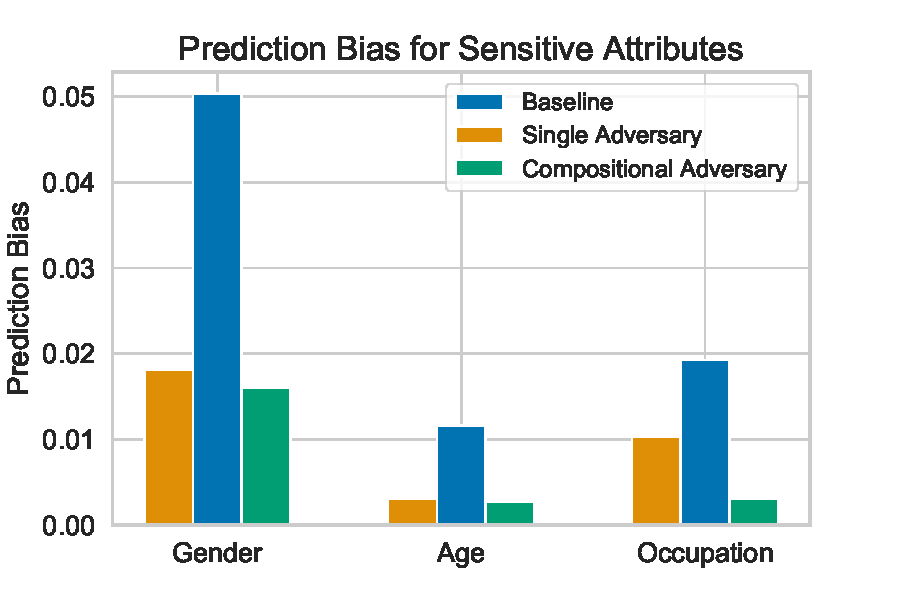
\includegraphics[width=1\linewidth]{icml2019_style/paper/plots/movielens1m_pred_bias.pdf}
    \caption{Prediction Bias for different Sensitive Attributes under three settings in MovieLens1M.}
    \label{fig:pred_bias}
\end{figure}

\begin{figure}
    \centering
    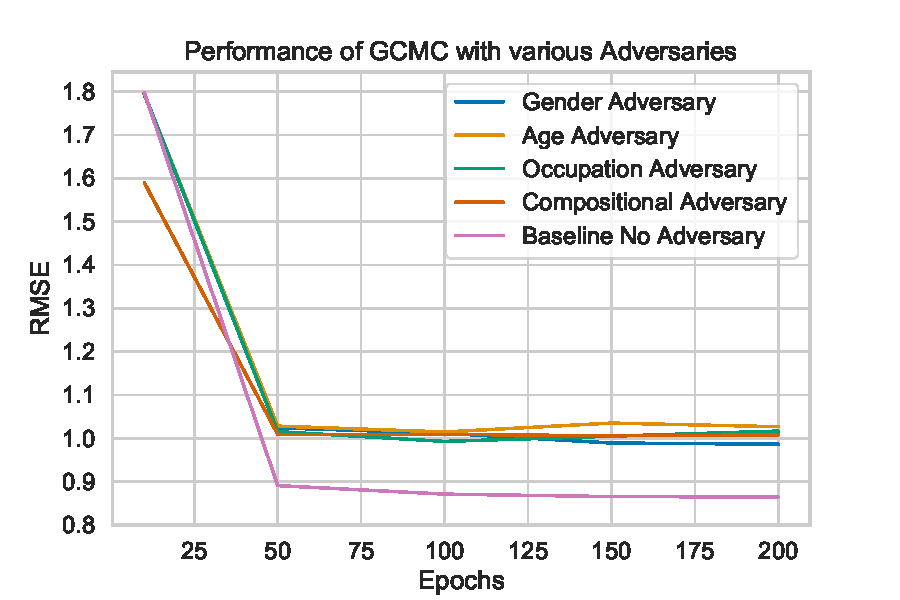
\includegraphics[width=1\linewidth]{icml2019_style/paper/plots/movielens1m_rmse.pdf}
    \caption{Performance of GCMC style encoder on MovieLens1M}
    \label{fig:rmse}
\end{figure}

\cut{
\begin{figure}
    \centering
    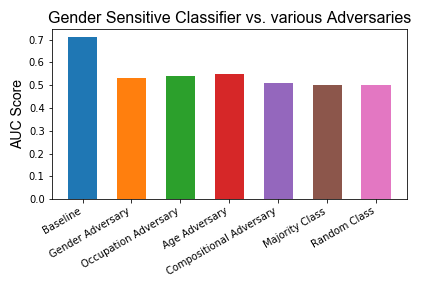
\includegraphics[width=1\linewidth]{icml2019_style/paper/plots/movielens1m_gender_auc.png}
    \caption{Gender Classifier AUC score versus various adversaries.}
    \label{fig:gender_f1}
\end{figure}

\begin{figure}
    \centering
    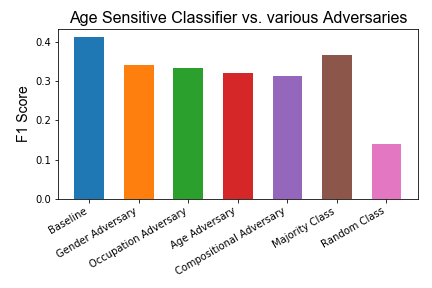
\includegraphics[width=1\linewidth]{icml2019_style/paper/plots/movielens1m_ageF1.png}
    \caption{Age Classifier F1 score versus various adversaries.}
    \label{fig:age_f1}
\end{figure}

\begin{figure}
    \centering
    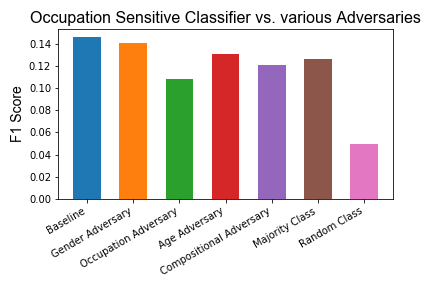
\includegraphics[width=1\linewidth]{icml2019_style/paper/plots/movielens1m_occF1.png}
    \caption{Occupation Classifier F1 score versus various adversaries.}
    \label{fig:occ_f1}
\end{figure}
}
\begin{figure}
    \centering
    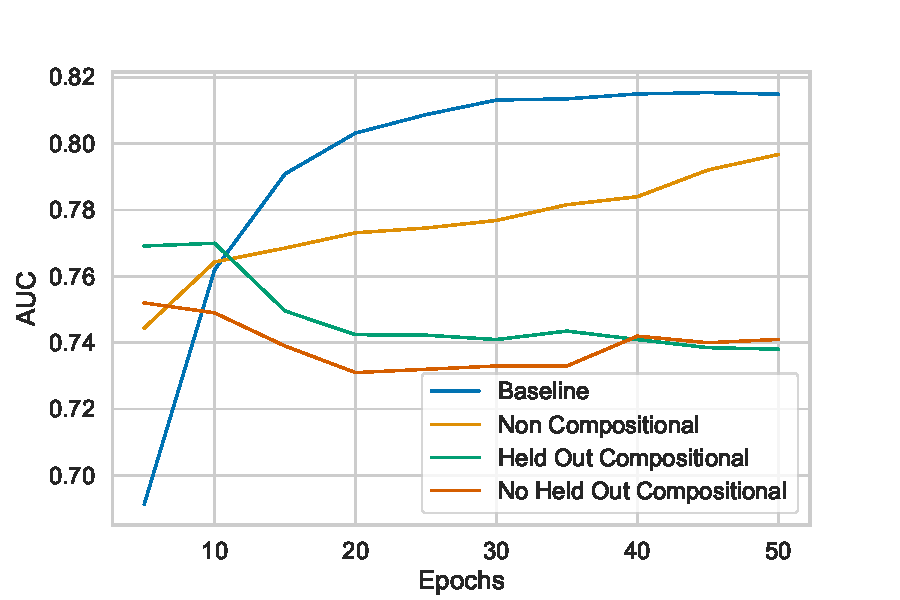
\includegraphics[width=1\linewidth]{icml2019_style/paper/plots/reddit_enc_auc.pdf}
    \caption{Reddit Encoder AUC score versus various Adversaries}
    \label{fig:reddit_enc_auc}
\end{figure}

\begin{figure}
    \centering
    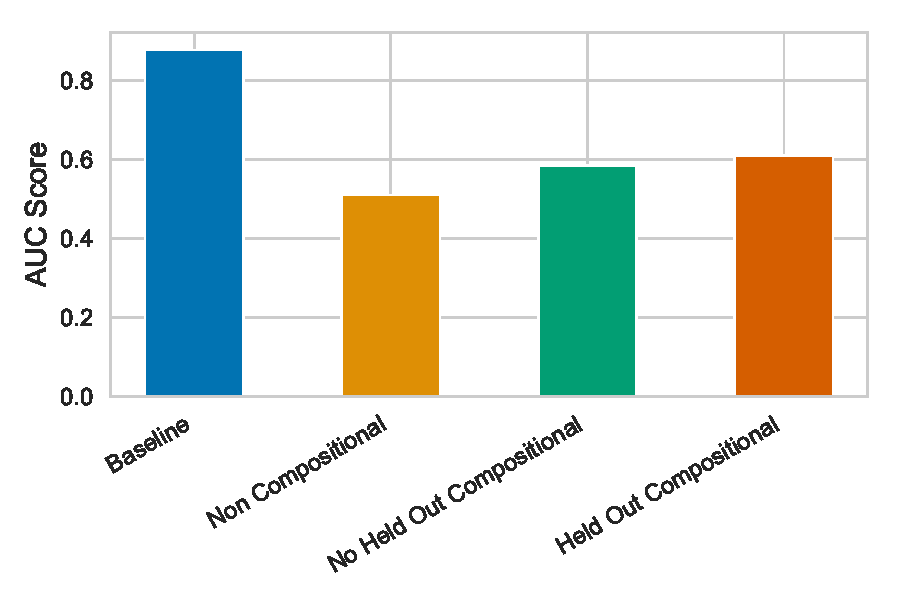
\includegraphics[width=1\linewidth]{icml2019_style/paper/plots/reddit_auc.pdf}
    \caption{Average Subreddit Classifier AUC score versus various Adversaries}
    \label{fig:reddit_auc}
\end{figure}

\begin{table*}[t]
\caption{Number of Head and Tail Nodes and Edges for each dataset. For FB15k-237 there is no distinction between Head and Tail nodes. We further indicate whether the sensitive attributes in each dataset are binary,multiclass or a combination of both.}
\label{sample-table}
\vskip 0.15in
\begin{center}
\begin{small}
\begin{sc}
\begin{tabular}{lcccccr}
\toprule
Dataset & \multicolumn{1}{p{1.5cm}}{\centering Head \\ Nodes} & \multicolumn{1}{p{1.5cm}}{\centering Tail \\ Nodes} & Edges & \multicolumn{1}{p{1.5cm}}{\centering Binary \\ Attributes?} & \multicolumn{1}{p{1.5cm}}{\centering Multiclass \\ Attributes?} \\
\midrule
FB15k-237    & 14,541& - & 237 &$\surd$ & $\times$ \\
MovieLens1M & 6,040&  3,900& 1,000,209&$\surd$ &$\surd$\\
Reddit Comments    & 366,797& 18938 &7,255,096 &$\surd$ & $\times$ \\
\bottomrule
\end{tabular}
\end{sc}
\end{small}
\end{center}
\vskip -0.1in
\label{dataset_stats}
\end{table*}



\begin{table*}[t]
\caption{Performance of Sensitive Attribute Classifiers versus various Adversaries. For Gender the score is AUC while for Age and Occupation the score is micro averaged F1. The columns represent the different adversaries while the rows are the respective classifiers.}
\label{sample-table}
\vskip 0.15in
\begin{center}
\begin{small}
\begin{sc}
\begin{tabular}{lccccccr}
\toprule
MovieLens1M & \multicolumn{1}{p{1.5cm}}{\centering Baseline \\ No Adversary} & \multicolumn{1}{p{1.5cm}}{\centering Gender \\ Adversary} & \multicolumn{1}{p{1.5cm}}{\centering Age \\ Adversary} & \multicolumn{1}{p{1.5cm}}{\centering Occupation \\ Adversary}&\multicolumn{1}{p{1.5cm}}{\centering Comp. \\ Adversary} & \multicolumn{1}{p{1.5cm}}{\centering Majority \\ Classifier} & \multicolumn{1}{p{1.5cm}}{\centering Random \\ Classifier} \\
\midrule
Gender Classifier   & 0.712& 0.532& 0.541 & 0.551 & 0.511 & 0.5 & 0.5 \\
Age Classifier   & 0.412 & 0.341& 0.333 & 0.321 & 0.313 & 0.367 & 0.141\\
Occupation Classifier     & 0.146 & 0.141& 0.108 & 0.131 & 0.121 & 0.126 & 0.05 \\

\bottomrule
\end{tabular}
\end{sc}
\end{small}
\end{center}
\vskip -0.1in
\end{table*}


\begin{table}[t]
\caption{FB15k-237 AUC scores for the top 3 entity types as sensitive attributes. }
\label{sample-table}
\vskip 0.15in
\begin{center}
\begin{small}
\begin{sc}
\begin{tabular}{lcccr}
\toprule
FB15k-237 & \multicolumn{1}{p{1.5cm}}{\centering Baseline \\ No Adversary} & \multicolumn{1}{p{1.5cm}}{\centering Non \\ Comp. Adversary} & \multicolumn{1}{p{1.5cm}}{\centering Comp. \\ Adversary} \\
\midrule
Attribute 0    &0.97& 0.94& 0.81  \\
Attribute 1 & 0.99& 0.90& 0.80\\
Attribute 2   & 0.98&  0.95& 0.85 \\
Mean Rank &285& 5505& 542 \\
\bottomrule
\end{tabular}
\end{sc}
\end{small}
\end{center}
\vskip -0.1in
\end{table}


\section{Conclusion}
We introduce an adversarial framework to enforce compositional fairness constraints on graph embeddings. 
Our approach uses a bank of adversarial filters to optionally enforce fairness constraints over a set of possible sensitive attributes.
Our work sheds light on how fairness can be enforced in graph representation learning, and our compositional approach highlights how fairness could be deployed in a real-word, user-driven setting, where it is necessary to optionally enforce a large number of invariance constraints over learned graph representations.
%Our preliminary results highlight the tradeoff between the flexibility afforded by this compositional approach, and the model performance. 

\bibliography{bibliography.bib}
\bibliographystyle{icml2019}




\end{document}


% This document was modified from the file originally made available by
% Pat Langley and Andrea Danyluk for ICML-2K. This version was created
% by Iain Murray in 2018, and modified by Alexandre Bouchard in
% 2019. Previous contributors include Dan Roy, Lise Getoor and Tobias
% Scheffer, which was slightly modified from the 2010 version by
% Thorsten Joachims & Johannes Fuernkranz, slightly modified from the
% 2009 version by Kiri Wagstaff and Sam Roweis's 2008 version, which is
% slightly modified from Prasad Tadepalli's 2007 version which is a
% lightly changed version of the previous year's version by Andrew
% Moore, which was in turn edited from those of Kristian Kersting and
% Codrina Lauth. Alex Smola contributed to the algorithmic style files.
